\documentclass[11pt]{article}
\usepackage{amsmath}
\usepackage{algpseudocode,algorithm}
\usepackage{subfigure}
\usepackage{graphicx}
\usepackage{psfrag,color}
\usepackage{fullpage}
\usepackage{epsfig}
\usepackage{amssymb}
\usepackage{titlesec}
\usepackage{minted}

\titleformat{\section}
  {\normalfont\large\bfseries}   
  {}
  {0pt}
  {}

\titleformat{\subsection}
  {\normalfont\bfseries}   
  {}
  {0pt}
  {}

\setlength{\textwidth}{6.5in}
\setlength{\oddsidemargin}{0.0in}
\setlength{\textheight}{9.0in}
\setlength{\parindent}{0in}

\renewcommand\arraystretch{2.4}

\renewcommand{\baselinestretch}{1.2}
\newcommand{\problem}[1]{ \medskip \pp $\underline{\rm Problem\ #1}$\\ }

\pagestyle{empty}

\def\pp{\par\noindent}
\DeclareMathOperator{\E}{\mathbb{E}}
\begin{document}

\centerline{\{\bf Amy Qi, xq2224\}}
\centerline{\bf Homework 2 Solutions}
\centerline{\bf W4771 Machine Learning --- Fall 2023}

\bigskip 
\bigskip

\section*{Problem 1}
\subsection*{(a)}
\begin{minted}[breaklines]{python}
import pickle
wine = pickle.load(open('wine.pkl', 'rb'))
print(wine['data'].shape, wine['testdata'].shape)
# prints (88, 13) (90, 13)
\end{minted}
Observe that the dataset is fairly small. It makes sense to use leave-one-out cross validation given the small dataset so that we can reuse most of the training data. \\
To test which two features are the most accurate, try all combinations of two features in the training dataset, i.e., extract all combinations of two columns in the dataset. \\
For each combination, perform LOO cross validation, i.e., save one example (one row) for validation, and use the rest for training. \\
To evaluate which combination of two features is the best, keep track of the number of prediction error for each combination. This is done by tracking how many of the cross-validation records are classified wrong. The best combination is the one with the lowest count. \\
In this wine dataset, two features that give the optimal result as suggested by LOO cross validation are Alcohol (indexed 0) and Flavanoids (indexed 6). \\
Code attached below for details.
\begin{minted}[breaklines]{python}
################################################################################
# Part (a)

# learn() function for bivariate normal generative model
def learn(train_x, train_y, num_classes=3):
    train_x_f1 = train_x[:, 0]
    train_x_f2 = train_x[:, 1]
    return [(np.mean(train_y == k), np.mean(train_x_f1[train_y == k]), np.mean(train_x_f2[train_y == k]), np.cov(train_x_f1[train_y == k], train_x_f2[train_y == k])) for k in range(num_classes)]

# predict() function for bivariate normal generative model
def predict(params, test_x):
    all_log_posteriors = []
    for prior, mu1, mu2, cor in params:
        mat = np.array([[test_x[0]-mu1],[test_x[1]-mu2]])
        log_posterior = np.log(prior) - np.log(np.linalg.det(cor))/2 - (mat.T @ np.linalg.inv(cor) @ mat)/2
        all_log_posteriors.append(log_posterior)
    
    log_posteriors = np.array(all_log_posteriors)
    return np.argmax(log_posteriors, axis=0)

# function to select the best 2 features
def select_params(train_data, train_label):
    optimal_feat_idx = None
    min_err_count = 10000000 # some large number
    
    feat_idx = combinations(range(train_data.shape[1]), 2)
    for i in feat_idx:
        # make a deep copy
        X = np.array(train_data)

        # track number of correct predictions given the two features
        err_count = 0

        # select two features
        idx1 = slice(i[0], i[0]+1)
        idx2 = slice(i[1], i[1]+1)
        extracted = np.hstack((X[:, idx1], X[:, idx2]))

        # leave-one-out cross validation
        for j in range(extracted.shape[0]):
            val_test = extracted[j]
            val_test_label = train_label[j]
            mask = np.ones(extracted.shape[0], bool)
            mask[0] = 0
            val_train = extracted[mask]
            val_train_label = train_label[mask]
            
            model = learn(val_train, val_train_label)
            result = predict(model, val_test)[0]
            if(result != val_test_label):
                err_count += 1

        # check optimality
        if (min_err_count > err_count):
            min_err_count = err_count
            optimal_feat_idx = i
    return optimal_feat_idx

# driver code to get the result
train_data = np.array(wine['data'].astype(float))
train_label = np.array(wine['labels'])

select_params(train_data, train_label) # prints (0,6)
\end{minted}

\subsection*{(b)}
The final classifier uses Alcohol (indexed 0) and Flavanoids (indexed 6) as the two features selected. Training error rate for this model is $0.045454545454545456$ and testing error rate for this model is $0.07777777777777778$. Parameters for this bivariate normal generative model are
\begin{center}
    \begin{tabular}{*{20}{|c}}
      \hline
   & $\pi$ & $\mu_1$ & $\mu_2$ & $\Sigma_{1,1}$ & $\Sigma_{1,2}$ & $\Sigma_{2,1}$ & $\Sigma_{2,2}$ \\ 
  \hline
  class 0 & 330 & 13.771 & 3.008 & 0.236 & 0.062 & 0.062 & 0.123 \\ 
  \hline
  class 1 & 0.398 & 12.221 & 2.000 & 0.216 & 0.055 & 0.055 & 0.447 \\ 
  \hline
  class 2 & 0.273 & 13.127 & 0.776 & 0.242 & 0.053 & 0.053 & 0.092 \\ 
  \hline
    \end{tabular}
\end{center}
where $\pi$ is the prior probability, $\mu_1$ and $\mu_2$ are the means of the features, and $\Sigma_{i,j}$ demotes the $(i,j)$-th entry in the covariance matrix. \\
Code attached below for details.
\begin{minted}{python}
################################################################################
# Part (b)

train_data = np.array(wine['data'].astype(float))
train_label = np.array(wine['labels'])
test_data = np.array(wine['testdata'].astype(float))
test_label = np.array(wine['testlabels'])

extracted_train_data = np.column_stack((train_data[:, 0], train_data[:, 6]))
extracted_test_data = np.column_stack((test_data[:, 0], test_data[:, 6]))
model = learn(extracted_train_data, train_label)

print(model) # get the parameters for the model

train_err = 0
test_err = 0

# find training error rates
for i in range(extracted_train_data.shape[0]):
    pred = predict(model, extracted_train_data[i])[0]
    if (pred != train_label[i]):
        train_err += 1

train_error_rate = train_err/train_data.shape[0]
print(train_error_rate)

# find test error rates
for i in range(extracted_test_data.shape[0]):
    pred = predict(model, extracted_test_data[i])[0]
    if (pred != test_label[i]):
        test_err += 1

test_error_rate = test_err/test_data.shape[0]
print(test_error_rate)
\end{minted}

\newpage
\section*{Problem 2}
\subsection*{(a)}
Given the distribution, the optimal classifier $f^*$ should behave as below.
\begin{equation}
    \begin{cases}
        \text{if } x\leq 0.2, \text{predict } 0 \\
        \text{if } 0.2<x<0.8, \text{predict } 1 \\
        \text{if } x\geq 0.8, \text{predict } 0
    \end{cases}
\end{equation}
Thus the error rate of this optimal classifier is \\
% err[$f^*$]=Pr($f(X)\neq Y$)\\
% =Pr($f^*(x)=0,Y=1$)+Pr($f^*(x)=1, Y=0$)
\begin{equation}
    \begin{split}
        \text{err}[f^*(x)] &= \text{Pr}(f^*(X)\neq Y)\\
        &= \text{Pr}(f^*(X)=0, Y=1) + \text{Pr}(f^*(X)=1, Y=0) \\
        &= \text{Pr}(X\leq 0.2)*\text{Pr}(Y=1) + \text{Pr}(0.2<X<0.8)*\text{Pr}(Y=0) + \text{Pr}(X\geq 0.8)*\text{Pr}(Y=1) \\
        &= 0.2*0.25 + 0.6*0.4 + 0.2*0.3 \\
        &= 0.35
    \end{split}
\end{equation}

\subsection*{(b)}
Code attached below. 
\begin{minted}[breaklines]{python}
################################################################################
# Part (b)

def stump_err(t, a, b):
    if(a==1 and b==0):
        if(t<=t1):
            return 0.75*t + 0.25*(0.2-t) + 0.42
        elif(t<t2):
            return 0.4*(t-0.2) + 0.6*(0.8-t) + 0.21
        else:
            return 0.7*(t-0.8) + 0.3*(1-t) + 0.39
    else:
        if(t<=t1):
            return 0.25*t + 0.75*(0.2-t) + 0.38
        elif(t<t2):
            return 0.6*(t-0.2) + 0.4*(0.8-t) + 0.19
        else:
            return 0.3*(t-0.8) + 0.7*(1-t) + 0.41

print(f'T1: {stump_err(0.4,0,1)}') # prints T1: 0.47000000000000003
print(f'T2: {stump_err(0.5,0,1)}') # prints T2: 0.49000000000000005
print(f'T3: {stump_err(0.5,1,0)}') # prints T3: 0.51
\end{minted}
So the error rates of the three stumps are 0.47000000000000003, 0.49000000000000005 and 0.51. 

\subsection*{(c)}
The threshold parameter $t$ of the decision stump $T$ that yields the smallest error rate $err[f_T]$ is $0.2$. The exact error rate is $0.43$. Code attached below. Imports omitted.
\begin{minted}[breaklines]{python}
################################################################################
# Part (c)
def min_err(t):
    return min(stump_err(t,0,1), stump_err(t,1,0), stump_err(t,0,0), stump_err(t,1,1))

# Plotting code
t_vals = np.linspace(-0.2, 1.2, num=14001)
best_stump_err_rates = np.array([min_err(t) for t in t_vals])

plt.figure()
plt.plot(t_vals, best_stump_err_rates)
plt.xlabel('$t$')
plt.ylabel('best stump error rate with predicate $x \leq t$')
plt.savefig('error_rates.pdf', bbox_inches='tight')
plt.close()

# find smallest value
print(min_err(0.2))
\end{minted}

The plot showing the error rates is on the next page.
\begin{figure}
    \centering
    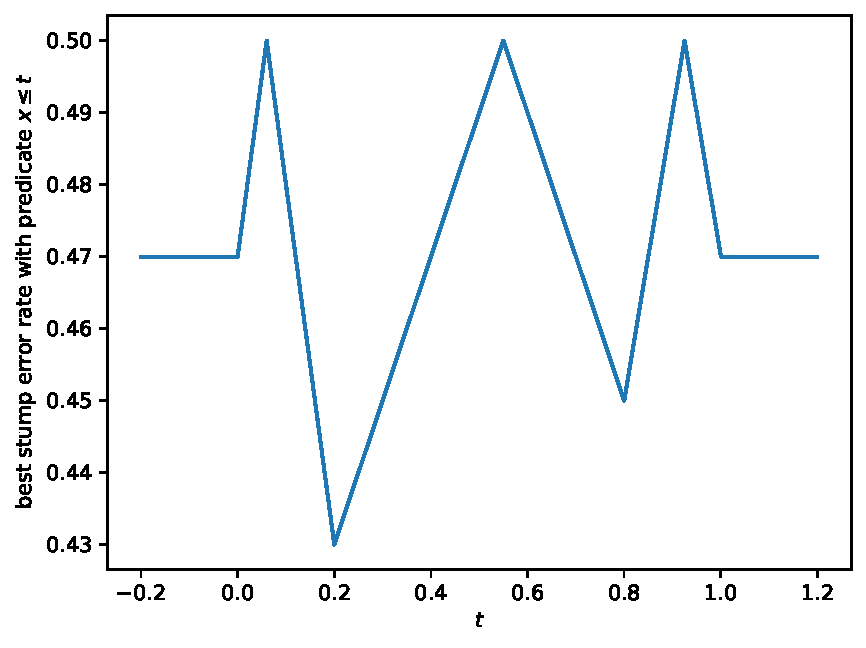
\includegraphics{images/2c.pdf}
\end{figure}

\newpage
\subsection*{(d)}
The decision stump obtained from this dataset is $T=$ "if $x\leq 0.75$ then return $0$, else return $1$." \\
It's training error rate is $0.176$. \\
Code attached below. Imports omitted.

\begin{minted}[breaklines]{python}
################################################################################
# Part (d)

def calc_err_rate(t, a, b, x, y):
    err = 0
    if(a==1 and b==0):
        for i in range(len(y)):
            if (x[i] <= t and y[i] == 0):
                err += 1
            if (x[i] > t and y[i] == 1):
                err += 1
    else:
        for i in range(len(y)):
            if (x[i] <= t and y[i] == 1):
                err += 1
            if (x[i] > t and y[i] == 0):
                err += 1
    return err/len(y)

# Function to implement
def find_best_stump(x,y):
    t = 0
    a = 0
    b = 0
    train_err_rate = 1
    for t_val in x:
        err01 = calc_err_rate(t_val, 0, 1, x, y)
        err10 = calc_err_rate(t_val, 1, 0, x, y)
        err_rate = min(err01, err10)
        
        if(err_rate < train_err_rate):
            t = t_val
            train_err_rate = err_rate
            if (err_rate == err01):
                a=0
                b=1
            else:
                a=1
                b=0
    
    return (t, a, b, train_err_rate)

x = np.array([0.1, 0.15, 0.2, 0.25, 0.3, 0.35, 0.4, 0.45, 0.5, 0.55, 0.6, 0.65, 0.7, 0.75, 0.8, 0.85, 0.9 ])
y = np.array([0, 1, 0, 0, 0, 1, 0, 0, 0, 1, 0, 0, 0, 0, 1, 1, 1])
t, a, b, train_err = find_best_stump(x, y)
print(f'{(t,a,b)}, {train_err:.3}') # prints (0.75, 0, 1), 0.176
\end{minted}

\subsection*{(e)}
The two plots obtained from this process are shown on the next page.
\begin{figure}
    \centering
    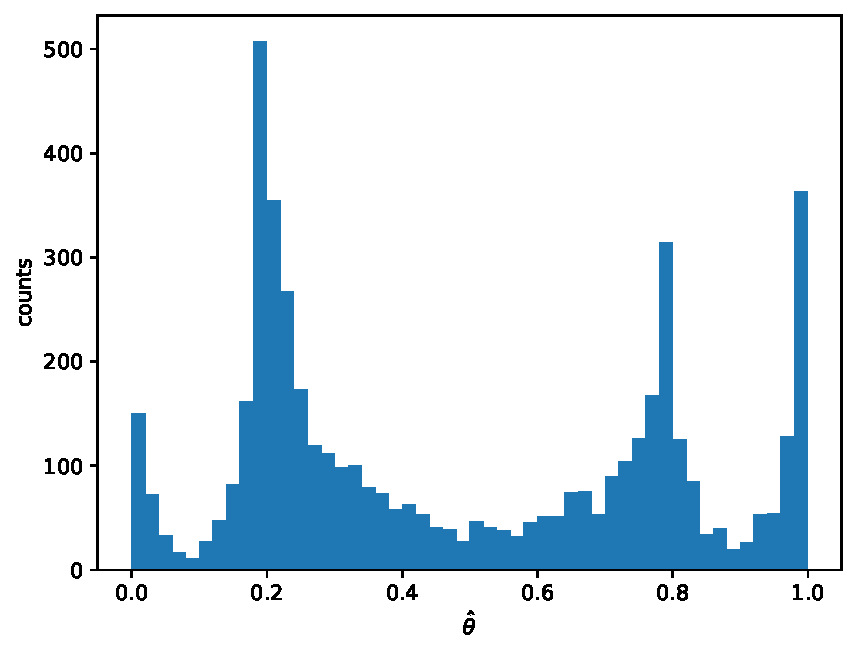
\includegraphics{images/2fthreshold.pdf}
\end{figure}

\begin{figure}
    \centering
    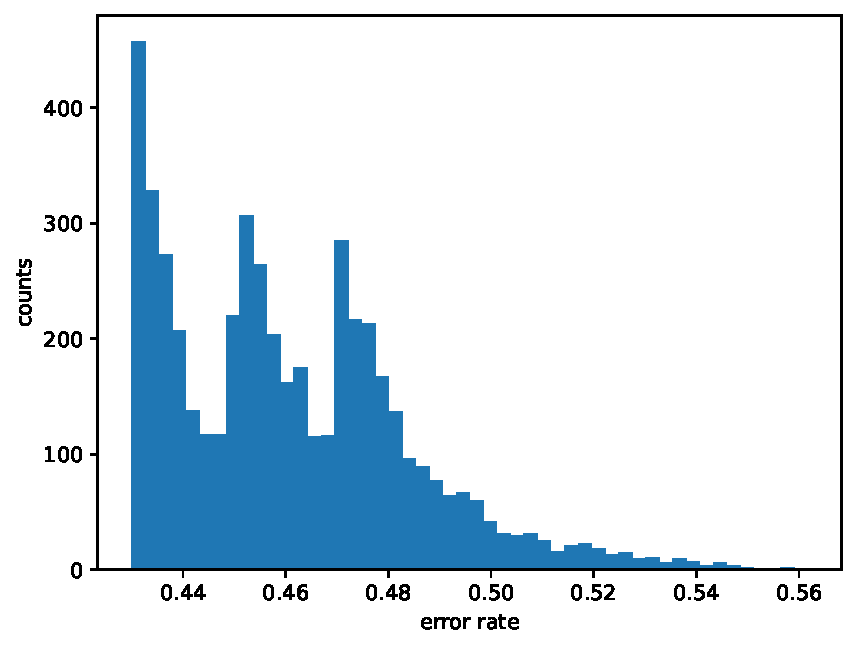
\includegraphics{images/2ferror.pdf}
\end{figure}

\newpage
\subsection*{(f)}
There are four peaks in the histogram for $t$, which are approximately located at $0$, $0.2$, $0.8$ and $1.0$. If we go back to the graph acquired in problem 2(c), these are the values where the optimal stumps that minimizes the error rates are found. \\
Now check the histogram for error rates. The first peak appears around $0.43$, which correspond to the minimum error rate when $t=0.2$ in the graph in 2(c). Similarly, the second peak at around $0.45$ corresponds to the min error rate at $t=0.8$ in the graph in 2(c), and the third peak at round $0.47$ corresponds to the min error rate at $t=0$ and $t=1$ in the graph in 2(c). \\
This means that, by simulating the distribution set up for the problem 2(a) to 2(c), we observe the pattern that matches our calculation for 2(c). Namely, the optimal stumps that minimizes the error rates are derived at $t=0$, $t=0.2$, $t=0.8$ and $t=1$. \\
However, since the dataset for each iteration is randomly generated, $Pr(Y=1|X=x)$ might deviate slightly, which is why we see four peaks (local minimum) instead of just the peak for $0.2$ (global minimum). The deviation leads to change of slope for the lines in 2(c), and this change of slope might lead to the global minimum shifting from one local minimum to another. Also, the noises in the graphs in 2(e) exist because of this random generation of data as well. \\
The piece of code responsible for generating the data is
\begin{minted}{python}
def generate_data(n):
    x = np.random.rand(n)
    z = np.random.rand(n)
    y = np.zeros(n)
    y[x <= t1] = z[x <= t1] <= p0
    y[(x > t1) * (x < t2)] = z[(x > t1) * (x < t2)] <= p1
    y[x >= t2] = z[x >= t2] <= p2
    return (x,y)
\end{minted}
Graphs attached below for reference.
\begin{figure}[htp]
    \centering
    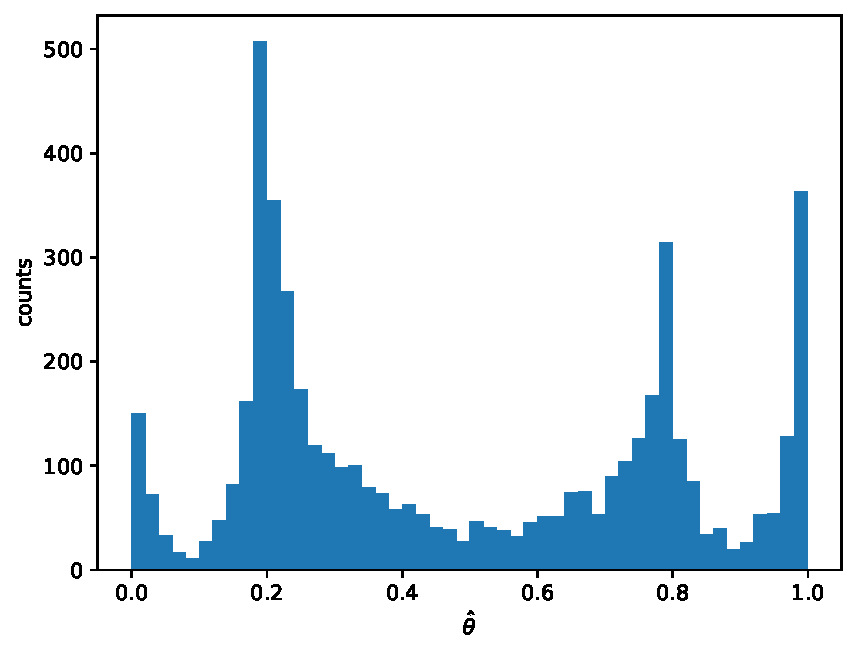
\includegraphics[width=.33\textwidth]{images/2fthreshold.pdf}\hfill
    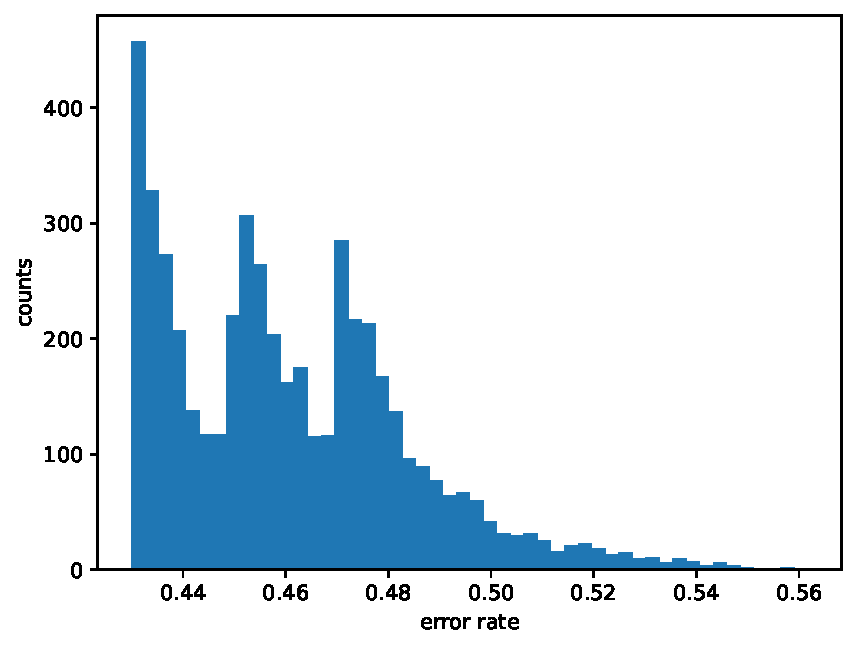
\includegraphics[width=.33\textwidth]{images/2ferror.pdf}\hfill
    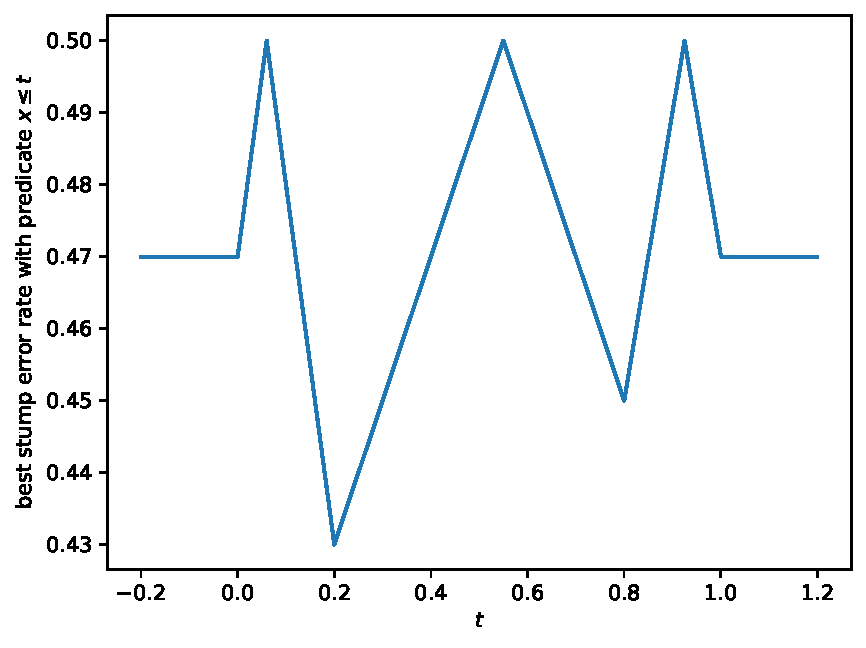
\includegraphics[width=.33\textwidth]{images/2c.pdf}
\end{figure}
% \begin{figure}[htp]
%     \centering
%     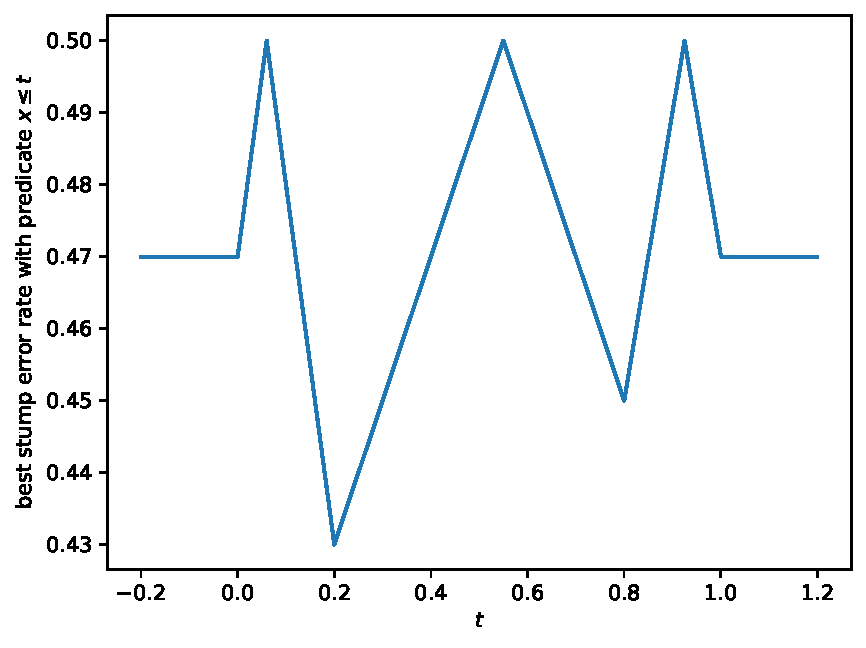
\includegraphics[width=.45\textwidth]{images/2c.pdf} \hfill
%     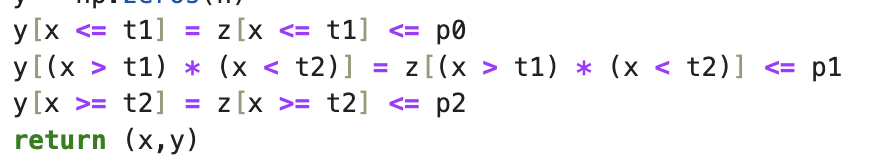
\includegraphics[width=.45\textwidth]{images/2fcode.png}
% \end{figure}

\newpage
\section*{Problem 3}
\subsection*{(a)}
The slope and intercept of each case are listed in the table below. Code attached to the end of this subproblem.

\begin{center}
    \begin{tabular}{*{20}{|c}}
      \hline
   & \textbf{lcavol} & \textbf{lweight} & \textbf{age} & \textbf{lbph} & \textbf{svi} & \textbf{lcp} & \textbf{gleason} & \textbf{pgg45} \\ 
  \hline
  \textbf{slope}& 0.713 & 1.23 & 0.0366 & 0.217 & 1.60 & 0.422 & 0.583 & 0.0185 \\ 
  \hline
  \textbf{intercept} & 1.52 & -2.01 & 0.0795 & 2.44 & 2.09 & 2.54 & -1.48 & 1.97 \\ 
  \hline
    \end{tabular}
\end{center}

\begin{minted}[breaklines]{python}
################################################################################
# Part (a)

data = np.array(prostate['data'])
s = data.shape[0]
result = []

for i in range(data.shape[1]-1):
    idx = slice(i, i+1)
    avg_x = np.average(data[:,idx])
    avg_x_squared = np.average(np.square(data[:,idx]))
    reshaped = data[:,idx].reshape(67,)
    avg_xy = np.dot(reshaped, lpsa)/s
    avg_y = np.average(lpsa)
    m = (avg_xy - avg_x * avg_y)/(avg_x_squared - avg_x**2)
    b = avg_y - m * avg_x
    result.append((f'{m:.3}', f'{b:.3}'))

print(result)
# prints [('0.713', '1.52'), ('1.23', '-2.01'), ('0.0366', '0.0795'), ('0.217', '2.44'), ('1.6', '2.09'), ('0.422', '2.54'), ('0.583', '-1.48'), ('0.0185', '1.97')]
\end{minted}

\subsection*{(b)}
The intercept is 0.429 and the coefficients are 
\begin{center}
    \begin{tabular}{*{20}{|c}}
      \hline
   \textbf{lcavol} & \textbf{lweight} & \textbf{age} & \textbf{lbph} & \textbf{svi} & \textbf{lcp} & \textbf{gleason} & \textbf{pgg45}\\ 
  \hline
  0.577 & 0.614 & -0.019 & 0.145 & 0.737 & -0.206 & -0.0295 & 0.00947  \\ 
  \hline
    \end{tabular}
\end{center}

Code used for calculation attached below.
\begin{minted}[breaklines]{python}
################################################################################
# Part (b)

data = np.array(prostate['data'])
A = data[:, [0,1,2,3,4,5,6,7]]
Astar = np.hstack((A,np.ones([A.shape[0],1], A.dtype)))
b = data[:, 8]
x = np.linalg.lstsq(Astar, b, rcond=None)
for num in x[0]:
    print(f'{num:.3}')
\end{minted}

\newpage
\section*{Problem 4}
\subsection*{(a)}
The affine function is $Y=X_1$.\\
According to the normal equations,
\begin{equation}
    \begin{split}
        m &= \frac{avg(xy)-avg(x) avg(y)}{avg(x^2)-avg(x)^2} \\
        &= \frac{\E(xy)-\E(x)\E(y)}{\E(x^2)-\E(x)^2}\\
        &= \frac{\E(\frac{3}{2}X_1^2-\frac{3}{4}X_1X_2)-\E(X_1)\E(\frac{3}{2}X_1-\frac{3}{4}X_2)}{\E(X_1^2)-\E(X_1)^2} \\
        &= \frac{\frac{3}{2}\E(X_1^2)-\frac{3}{4}\E(X_1X_2)-\frac{3}{2}\E (X_1)^2+\frac{3}{4}\E(X_1)\E(X_2)}{\E(X_1^2)-\E(X_1)^2} \\
        &= \frac{3}{2} + \frac{3}{4} * \frac{\E(X_1)E(X_2)-\E(X_1X_2)}{\E(X_1^2)-\E(X_1)^2} \\
        &= \frac{3}{2} + \frac{3}{4} * \frac{-cov(X_1X_2)}{var(X_1)} \\
        &= \frac{3}{2} - \frac{3}{4} * \frac{2/3}{1} \\
        &= 1
    \end{split}
\end{equation}
Substitute $m=2$ in to the formula for $b$
\begin{equation}
    \begin{split}
        b &= avg(y)-m avg(x) \\
        &= \E(y) - \E(x) \\
        &= \E(\frac{3}{2}X_1-\frac{3}{4}X_2) -\E(X_1) \\
        &= \E (\frac{3}{2}X_1) - \E (\frac{3}{4}X_2) - \E(X_1) \\
        &= 0
    \end{split}
\end{equation}

\subsection*{(b)}
The affine function is $Y=\frac{1}{4}X_2$.\\
According to the normal equations,
\begin{equation}
    \begin{split}
        m &= \frac{avg(xy)-avg(x) avg(y)}{avg(x^2)-avg(x)^2} \\
        &= \frac{\E(xy)-\E(x)\E(y)}{\E(x^2)-\E(x)^2}\\
        &= \frac{\E(\frac{3}{2}X_1X_2-\frac{3}{4}X_2^2)-\E(X_2)\E(\frac{3}{2}X_1-\frac{3}{4}X_2)}{\E(X_2^2)-\E(X_2)^2} \\
        &= \frac{\frac{3}{2}\E(X_1X_2)-\frac{3}{4}\E(X_2^2)-\frac{3}{2}\E (X_1)\E(X_2)+\frac{3}{4}\E(X_2)^2}{\E(X_2^2)-\E(X_2)^2} \\
        &= -\frac{3}{4} + \frac{3}{2} * \frac{\E(X_1X_2)-\E(X_1)E(X_2)}{\E(X_2^2)-\E(X_2)^2} \\
        &= -\frac{3}{4} + \frac{3}{2} * \frac{cov(X_1X_2)}{var(X_2)} \\
        &= -\frac{3}{4} + \frac{3}{2} * \frac{2/3}{1} \\
        &= \frac{1}{4}
    \end{split}
\end{equation}
Substitute $m=2$ in to the formula for $b$
\begin{equation}
    \begin{split}
        b &= avg(y)-m avg(x) \\
        &= \E(y) - \frac{1}{4}\E(x) \\
        &= \E(\frac{3}{2}X_1-\frac{3}{4}X_2) - \frac{1}{4} \E(X_2) \\
        &= \E (\frac{3}{2}X_1) - \E (\frac{3}{4}X_2) - \frac{1}{4} \E(X_2) \\
        &= 0
    \end{split}
\end{equation}

\subsection*{(c)}
The affine function is $Y=\frac{3}{2}X_1-\frac{3}{4}X_2$.\\
To minimize the risk, we want to find the affine function $f(x)=m_1 X_1 + m_2 X_2 + b$ where $\E((f(x)-Y)^2)$ is minimized. \\
Substitute the $Y=\frac{3}{2}X_1-\frac{3}{4}X_2$ into the equation, we want to minimize $\E((m_1 X_1 + m_2 X_2 + b-\frac{3}{2}X_1+\frac{3}{4}X_2)^2)$ \\
Observe that if we put $m_1=\frac{3}{2}$, $m_2= -\frac{3}{4}$ and $b=1$, that formula evaluates to $0$. Since the expectation of a squared term cannot be smaller than $0$, this assignment must be at least as good as the optimal solution. Therefore, the affine function that yields the smallest mean squared error can be $Y=\frac{3}{2}X_1-\frac{3}{4}X_2$. 

\end{document}
